\section{INTRODUCTION}
System design has been carried out by using several software engineering techniques and some of the design methods and design diagrams are discussed in this chapter. The diagrams are designed according to the gathered requirements.

\section{DESIGN DIAGRAMS}
\subsection{TOP LEVEL NETWORK DIAGRAM}
\begin{figure}[H]	
	\centering
	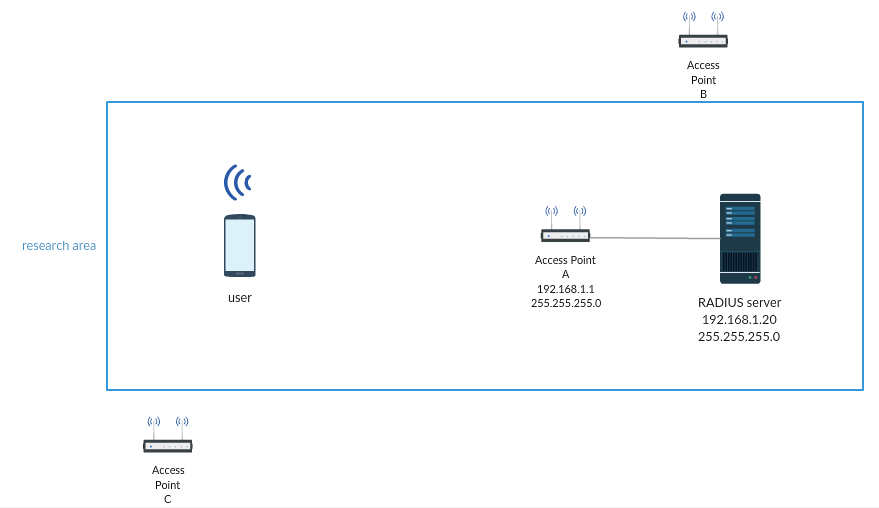
\includegraphics[width=0.9\textwidth]{toplevel_3.png}
	\caption{Top Level network Diagram}
\end{figure}

Three Wi-Fi access points (A,B and C) are fixed in three separate places and the access point A, which is enterprise support access point is connected to the RADIUS server by directly via network cable. 


\subsection{DATABASE DIAGRAM}
Proposed approach does not use complex database to authenticate users. Three main non-relational tables are being used to authenticate users.

\paragraph{}
Database design is carried out by using standard database normalization methods and there are two databases designed for the local database and the central database. Since the proposed solution uses RADIUS server for Wi-Fi user authentication, the MySQL database is running with authentication server to store all necessary data for user authentication.

\paragraph{}
within the Android application, data has been stored as shared preferences which contains user location information with respect to time.

\begin{figure}[h]	
	\centering
	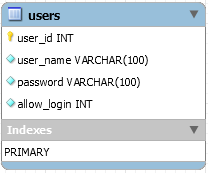
\includegraphics[width=0.3\textwidth]{users_table.png}
	\caption{Users table}
\end{figure}

\newpage
\paragraph{}
Users table contains all user information together with user name, password and special flag "allow login" to control user access by an administrator. This table is used by RADIUS server and also back end administration panel to manage user logins. 

\begin{figure}[h]	
	\centering
	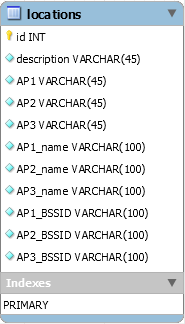
\includegraphics[width=0.3\textwidth]{locations_table.png}
	\caption{Location table}
\end{figure}
\paragraph{}
Location table is the place where all the data that has been collected by off-line training phase of the location fingerprinting technique is initially stored. This table contains all raw data of the Wi-Fi signal strengths (RSSI value) of each location of the research area. 

\begin{figure}[h]	
	\centering
	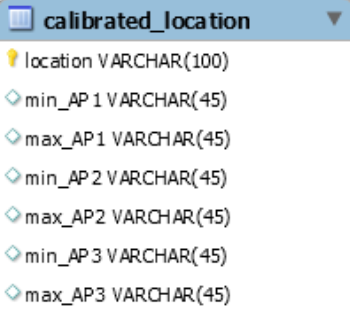
\includegraphics[width=0.3\textwidth]{calibrated_table.png}
	\caption{Calibrated location table}
\end{figure}

\newpage
\paragraph{}
This table view is generated by analyzing the location data table and retrieving the maximum and minimum RSSI value for each location for each Wi-Fi access point. This is the most important data source that is being used to authenticate user in on-line authentication phase of the location fingerprinting technique.

\subsection{ACTIVITY DIAGRAM}

\begin{figure}[h]	
	\centering
	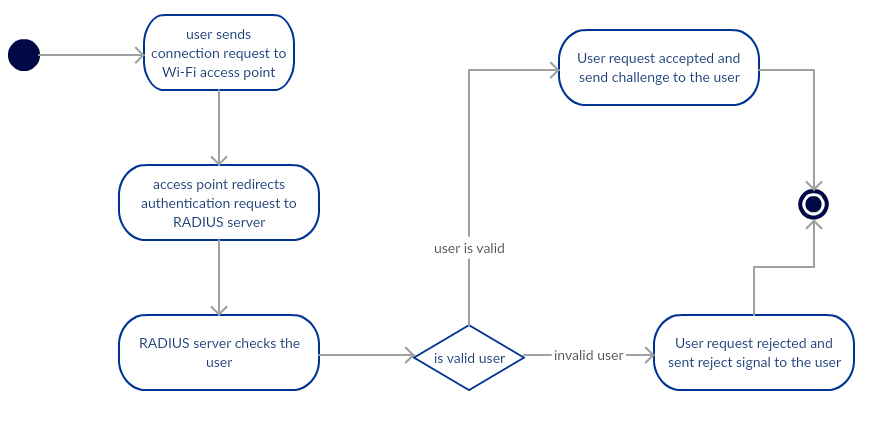
\includegraphics[width=1\textwidth]{activity_diagram.png}
	\caption{Activity diagram}
\end{figure}

\paragraph{}
Overall activity of the process is shown in activity diagram. This provides the general idea of the process. 

\newpage
\subsection{SYSTEM DESIGN}
Wi-Fi signal strength of each location of the identified area should be measured by using Wi-Fi signal strength measuring tool.
Since we know the exact location of the access point, we can measure the distance from each access point to pointed location.

\begin{figure}[h]	
	\centering
	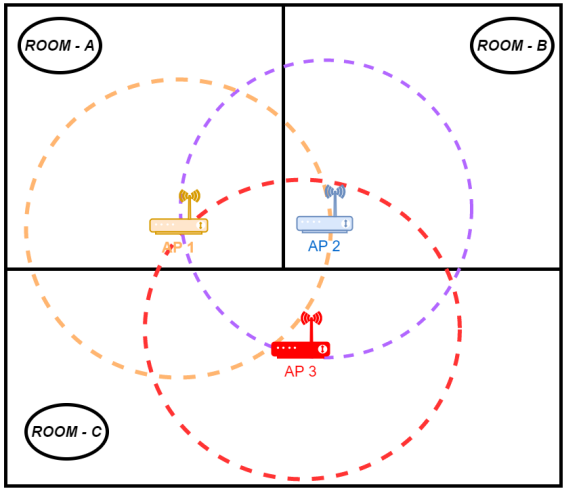
\includegraphics[width=0.8\textwidth]{signal_distribution.png}
	\caption{Signal Distribution of Wi-Fi access points}
\end{figure}

%\subsection{DATABASE DESIGN}
